% !TeX root = ../BA_main_englisch.tex
% !TeX spellcheck = en_GB
In this section we apply the methodology of section \ref{n_5_ml} to the case of $\Delta \mathrm{T} = 1$ with 5 Drive and Transducer qubits.
Contrary to $\Delta \mathrm{T} = 5$, the optimal System states cannot be reached.


\begin{figure}
	\centering
	\begin{subfigure}{0.85\textwidth}
		\centering
		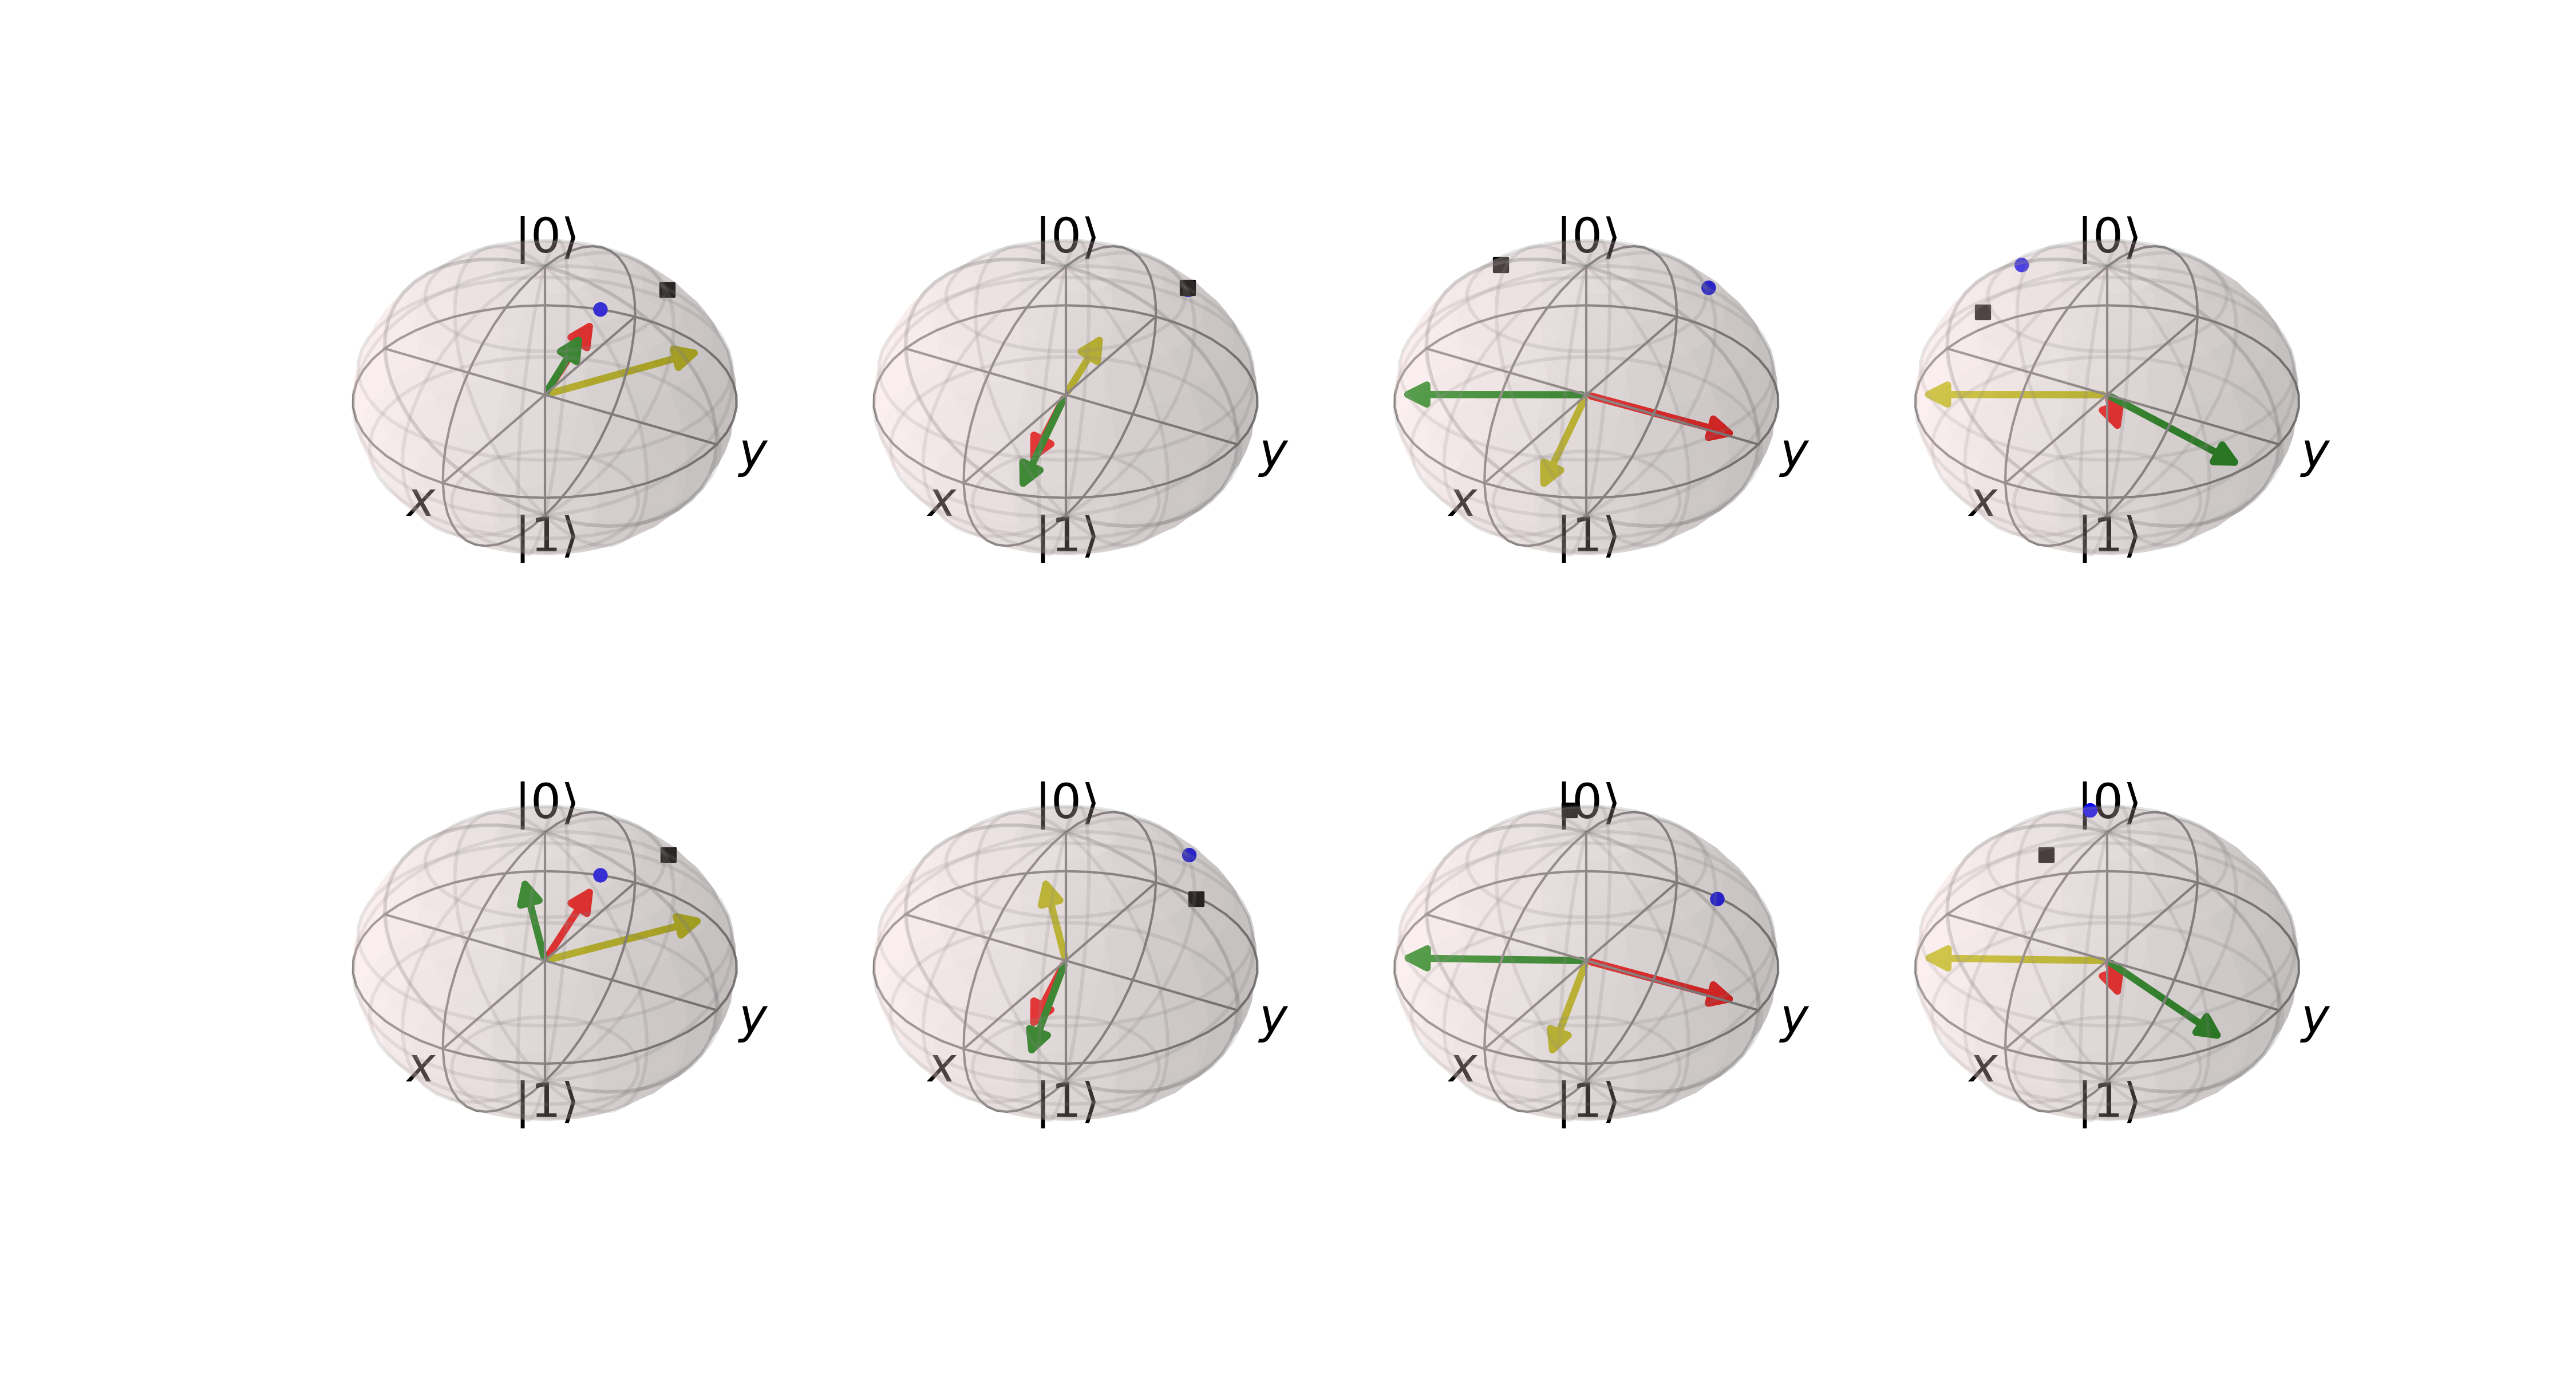
\includegraphics[width=\textwidth]{img/bloch_comp_1}
		\caption{$\Delta \mathrm{T} = 1: W_{opt} = 1.40, W_{pred} = 1.32$}
		\label{bloch_10553}
	\end{subfigure}
	\begin{subfigure}{0.85\textwidth}
		\centering
		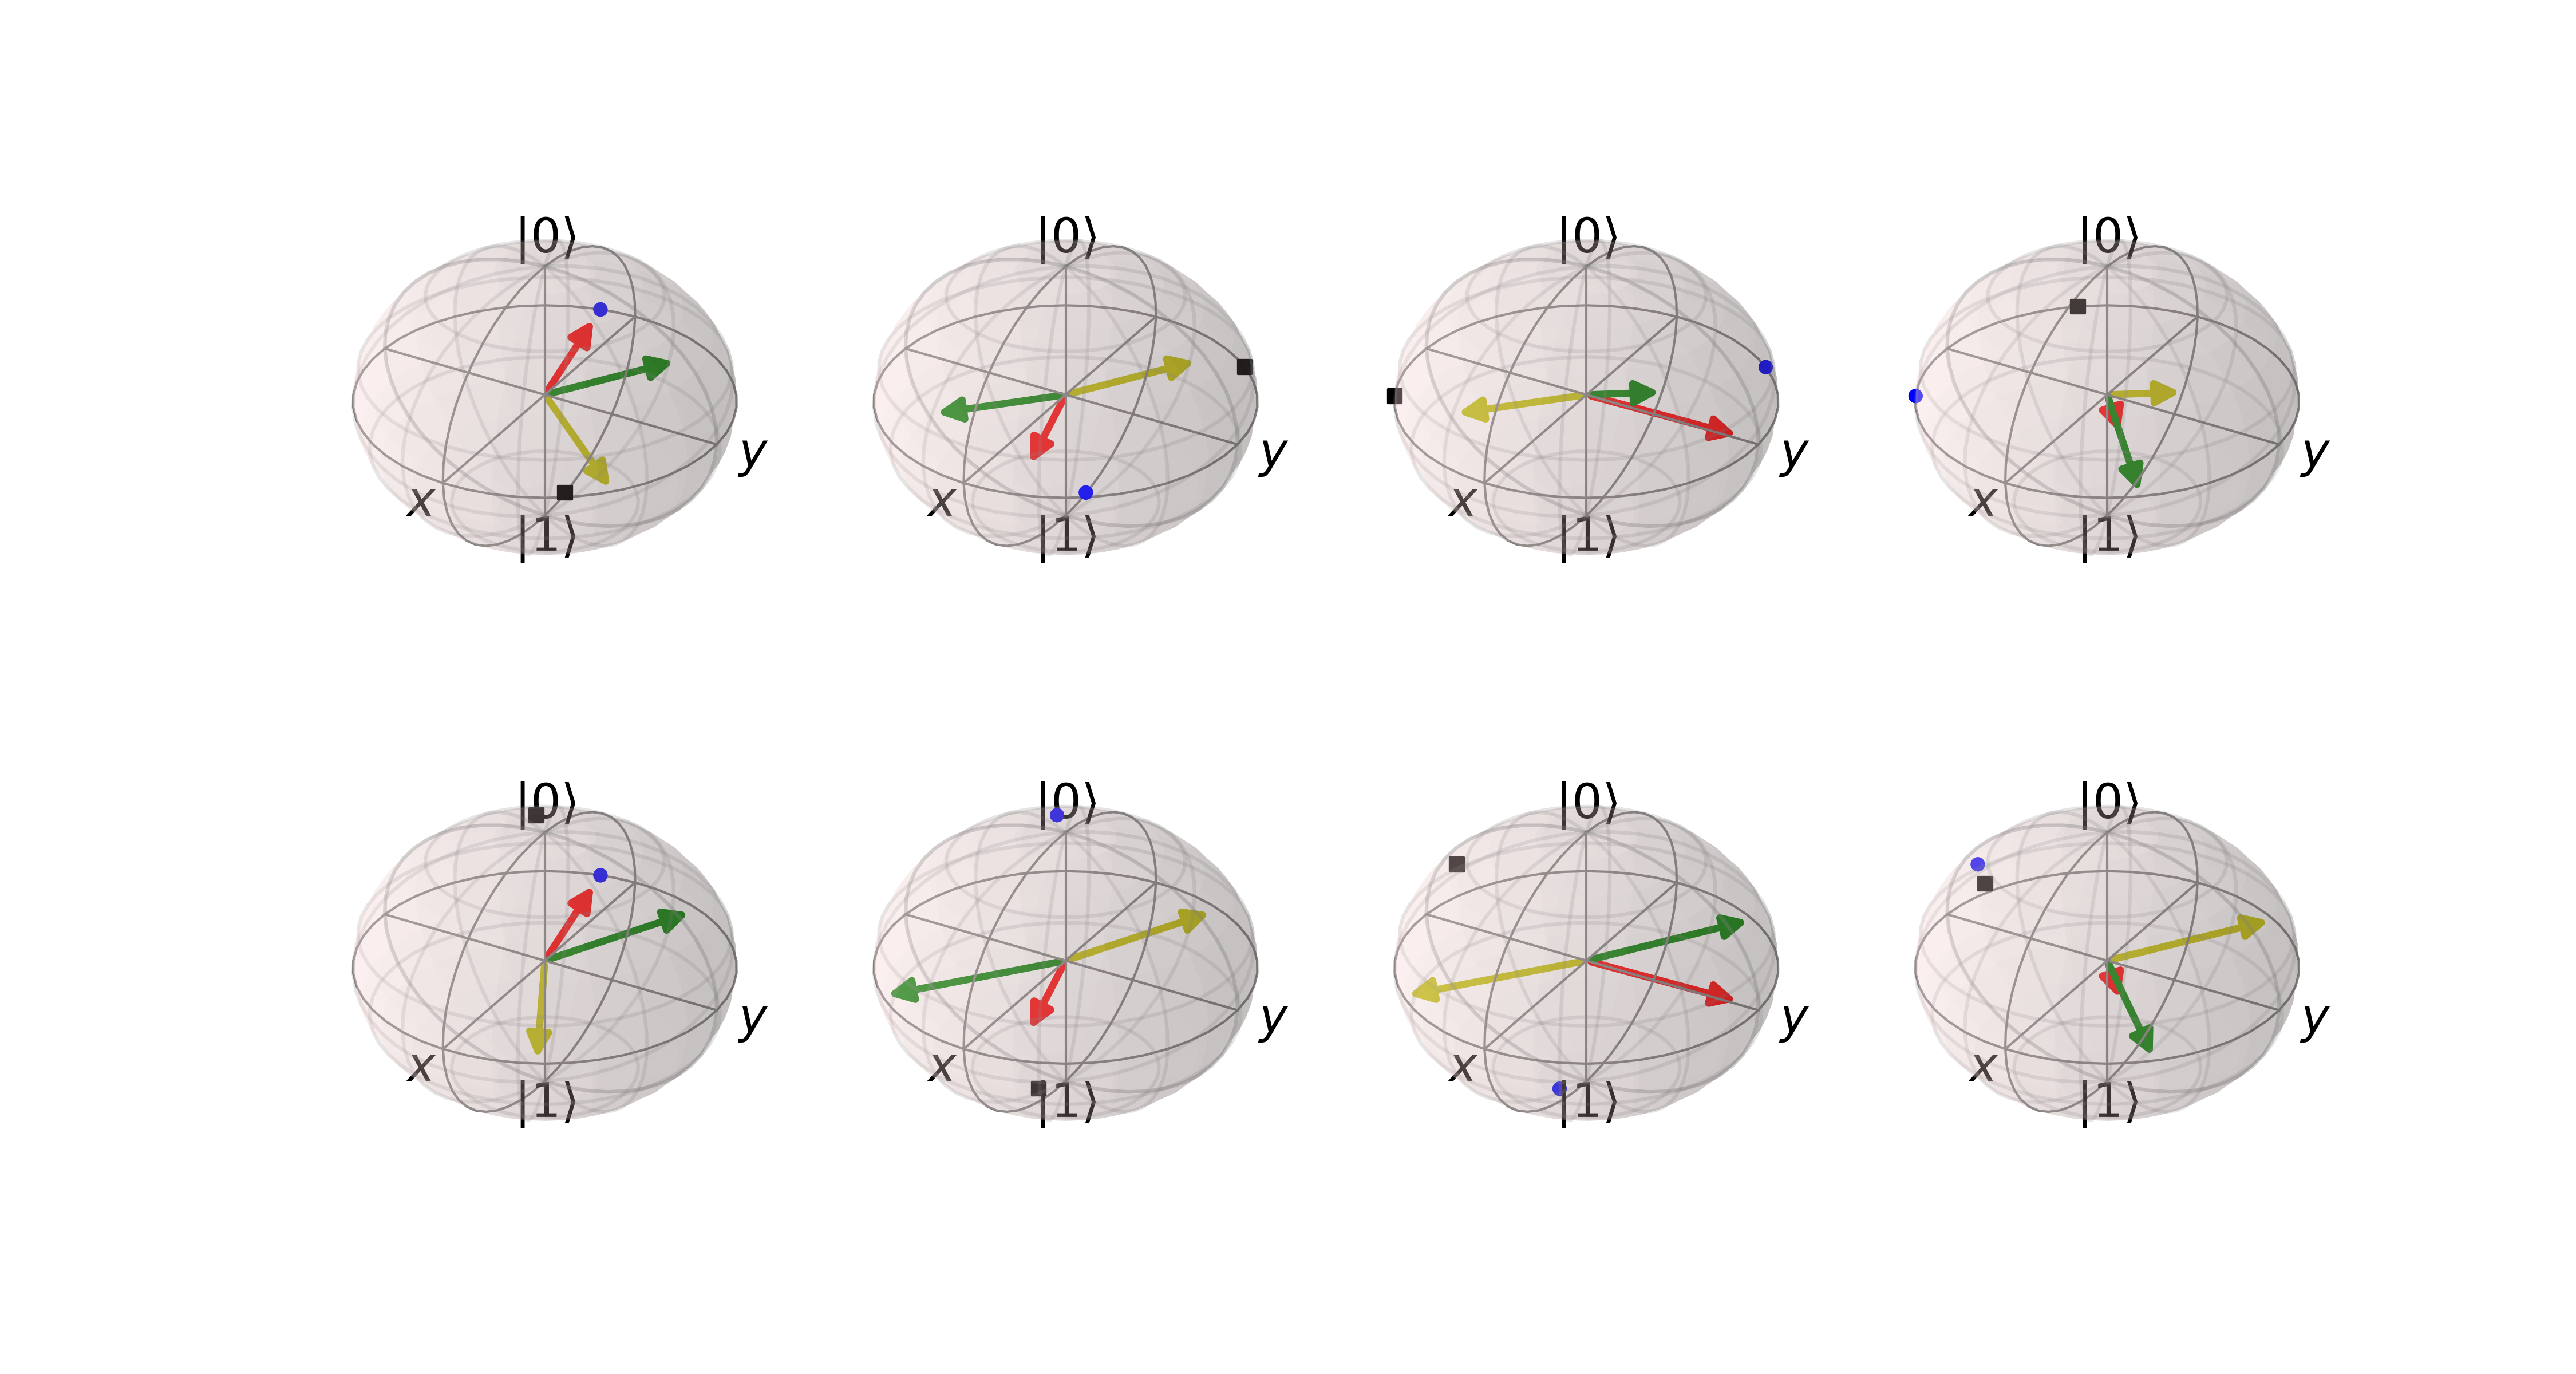
\includegraphics[width=\textwidth]{img/bloch_comp_5}
		\caption{$\Delta \mathrm{T} = 5: W_{opt} = 2.42, W_{pred} = 0.57$}
		\label{bloch_worst}
	\end{subfigure}
\end{figure}